\documentclass[12pt]{article}
\usepackage{geometry}
\geometry{a4paper, margin=2.5cm} 
%\usepackage[parfill]{parskip} 
\usepackage{amssymb}
\usepackage{amsmath}
\numberwithin{equation}{subsection}
\usepackage{amsthm}
\usepackage{setspace}
\usepackage{caption}
\usepackage{cancel}
%\setstretch{1.2}
\usepackage{graphicx}
\DeclareGraphicsExtensions{.pdf,.png,.jpg}
\usepackage{relsize}
%\usepackage{times}
\usepackage{hyperref}
\usepackage{letltxmacro}
\usepackage[reflist=true,style=windycity]{biblatex}
\addbibresource{refs.bib}
\urlstyle{same}

\newtheorem{theorem}{Theorem}
\newtheorem{proposition}{Proposition}

\theoremstyle{definition}
\newtheorem{definition}{Definition}
\newtheorem{algorithm}{Algorithm}


\DeclareMathOperator*{\argmax}{arg\,max}
\DeclareMathOperator*{\argmin}{arg\,min}



\begin{document}
\title{Characterizing nonatomic admissions markets}
\date{\today}
\author{Max Kapur\footnote{\emph{Email:} \href{mailto:maxkapur@snu.ac.kr}{maxkapur@snu.ac.kr}}}



\maketitle

\begin{abstract}
Abstract
\end{abstract}

\pagebreak
\tableofcontents

\pagebreak
\section{Introduction}
This article concerns decentralized admissions markets


In this study, I consider a special kind of admissions market that has not received much attention in the school-choice literature but approximates the admissions procedure used in many systems around the world. In this market, all schools have the same preference order, and students' preference orders are determined by the multinomial logit (MNL) choice model.

The primary reason for choosing this market is that it admits an expression for the demand that is invertible in the other parameters, allowing us to compute the equilibrium cutoffs analytically. We can also efficiently compute the gradient of the market parameters with respect to one another both in and out of equilibrium, which enables an interesting comparative analysis of the incentives available to schools under unconstrained school choice and when the market is confined to equilibrium by a deferred acceptance mechanism. Also, when the demand and cutoff vectors are known, one can solve for the preferability parameters, which yields a novel method of ranking schools' popularity and modeling their demand curves.

A single-score system may arise in one of several real-world scenarios. The most obvious case is when government regulations require schools to admit students solely on the basis of a standardized test. Alternatively, when students are scored using various dimensions of student characteristics such as test scores, GPA, and the quality of their letters of recommendation, it is common for these various dimensions to tightly correlate. If so, then principle component analysis can be used to determine a composite score whose order approximates the ordering of students at each university. Finally, in many public school systems, schools have \emph{no} preference order over the students; instead students take turns picking their favorite school in an order determined by random lottery, or (equivalently) the single tiebreaking mechanism is used to generate schools’ preference lists and the assignment of students to schools is computed using student-proposing DA \parencite[][]{whatmatters}. In this situation, the random numbers induce a single distribution of scores.

The MNL choice model represents a compromise between realism and computational tractability. In the general nonatomic school-choice problem, there are $|C|!$ possible preference orderings, and student preferences must be encoded as a probability vector of this length. A simple way to reduce this complexity is to choose a few ``representative'' preference lists, but this fails to account for the exponential number of ways in which an individual student may exchange the place of two schools within a primary list. In contrast, the MNL choice model assigns nonzero preferability to all possible preference lists while requiring only a single parameter for each school, and its parameters can be fitted via a number of known survey methodologies.\footnote{An interesting direction of future research would be to attempt to fit MNL parameters to student preference lists in a jurisdiction that uses deferred acceptance, like New York City.} The MNL choice model can also emulate to arbitrary precision the situation in which every student's preference list is \emph{identical}, by letting each school's preferability parameter differ from the next by a large order of magnitude. 

\subsection{Organization}
The body of this article is divided into two sections. The first (\S\ref{interpeqinadmmkts}) establishes preliminary results concerning a certain notion of equilibrium in nonatomic admissions markets, whose several possible interpretations include stable assignment. While this section's foundation is a result of Azevedo and Leshno \parencite*{supplydemandfw} establishing the equivalence of stable matchings and Walrasian equilibrium in matching markets, I provide a straightforward proof. I also argue that even when we abandon the centralized school assignment mechanism implied by stable assignment algorithms in favor of a decentralized, iterative admissions market in which schools adjust their admissions standards in pursuit of a target class size, the same notion of equilibrium retains interpretive meaning. Moreover, I show that deferred acceptance algorithms are a special case of a price adjustment rule called t\^{a}tonnement, which is known to converge to equilibrium under certain conditions, and whose iterates behave like the price paths of perishable goods. 

In the second section (\S\ref{singlescoremodel}), I apply the results above to a parameterized admissions market that I call the single-score market with multinomial logit student preferences. This model is chosen for its computational tractability. Unlike the nonatomic markets theorized by previous work, in which computing the equilibrium requires evaluating a demand function that is exponentially complex in the number of schools, the model considered here admits a piecewise linear demand function, and each school's cutoff at equilibrium can be expressed as the solution of a triangular linear system. In this context, comparative statics at the equilibrium can be computed analytically. I also provide an inverse optimization procedure that computes the preferability parameter for each school given the cutoff and demand vectors, and I apply the procedure to a dataset of 677 American colleges. Despite the noisy input data and the model's intrinsic simplicity, this procedure yields a familiar ranking of top universities, and does so without using the costly opinion surveys or data on alumni outcomes that newspapers traditionally use to rank schools. Furthermore, it provides an estimate of each school's demand curve, which could be a useful supplement to the logistic regression models that program planners currently use to predict their admissions yield.

\section{Model description} \label{singlescoremodel}
This article considers an admissions market with \underline{m}ultino\underline{m}ial logit student \underline{p}references and \underline{h}omogeneous \underline{s}coring (hereafter Memphis). The market consists of a finite set of schools $C = \{ 1\dots |C| \}$ and continuum of students having unit mass and Lebesgue measure $\eta$.

The market is characterized by four parameters:
\begin{enumerate}
\item The vector of school preferability parameters $\gamma \in [0, \infty)^C$. 
\item The score cutoff vector $p \in [0, 1]^C$. 
\item The demand vector $D \in [0, 1]^C$.
\end{enumerate}

Each student has a preference order $\succ_s$ over the set of schools. The preference lists are derived from the multinomial logit choice (MNL) model as follows: Each school has an associated quality parameter $\delta_c \in \mathbb{R}$. Each student perturbs the vector $\delta$ by a vector of random Gumbel variables, and the order established by the perturbed values is the student's preference order.

Letting $C^\# \subseteq C$ denote a student's consideration set---for example, the set of schools to which she is admitted. It can be shown that under MNL choice, the probability that she chooses to attend school $c \in C^\#$ is
\[\frac{\exp \delta_c}{\sum_{d \in C^\#} \exp \delta_d}\]
For the remainder of this article, let $\gamma_c \equiv \exp \delta_c > 0$ and $\Gamma = \sum_c \gamma_c$. Since the equation above is homogeneous in $\gamma$, we may assume without loss of generality that $\Gamma = 1$; however, I will resist this assumption, since in a large market, taking a larger $\Gamma$-value can yield more legible parameters. 

Each student also has a score $\theta \in [0,1]$. Schools prefer students with higher scores, and I assume that ties among students' scores occur with probability zero. Since this article considers only schools' ordinal preferences over students, I assume without loss of generality that students' scores are uniformly distributed. I also assume that the scores are independent of students' preference orders. Thus, the space of students is $C! \times [0, 1]$, and $\eta$ has full support, because the probability of a student having any given preference order is greater than zero. 

The market operates as follows. At the beginning of the admissions cycle, each school chooses a score cutoff $p_c \in [0, 1]$, which indicates the minimum score threshold such that a student having score $\theta$ is admitted to school $c$ if and only if $\theta \geq p_c$.  student observes her consideration set  $C^\# = \{c: \theta \geq p_c$ and enrolls in her favorite school. Then, each school observes its demand $D_c$, which represents the number of students who choose to enroll as a proportion of the total number of students in the market. That is, the demand for $c$  is the measure of students who are admitted to school $c$ and not admitted to any school that they prefer to $c$:
\begin{equation} \label{demanddefinition}
D_c \equiv \eta\left(s: c = \argmax_{\text{wrt } \succ_s} \left\{\hat c: \theta_{s\hat c} \geq p_{\hat c} \right\}\right)
\end{equation}
Observe that $D_c$ is determined entirely by $p$ and $\gamma$. $D_c$ is weakly decreasing in $p_c$ and weakly increasing in $p_{c'}$ for $c' \neq c$, and $p_c = 1 \implies D_c = 0$ regardless of the other schools' cutoffs.

In summary, the market is characterized

\subsection{Demand function}
Let us determine a closed-form expression for the demand function $D(\gamma, p)$ for a Memphis market. First, sort the schools by cutoff, so that
\[p_1 \leq p_2 \leq \dots \leq p_{|C|}\]
Ties may be broken arbitrarily, as discussed below. Since getting into school $c$ implies getting into any school whose cutoff is less than or equal to $p_c$, there are only $|C| + 1$ possible consideration sets for each student, as follow.
\begin{center}
\begin{tabular}{lll}
\textbf{Symbol} & \textbf{Consideration set} & \textbf{Probability} \\ \hline
$C_{[0]}$    & $\varnothing$    & $p_1$                  \\
$C_{[1]}$    & $\left\{ c_1 \right\}$    & $p_2 - p_1$               \\
$C_{[2]}$    & $\left\{ c_1, c_2 \right\}$    & $p_3 - p_2$               \\
$\vdots$ & $\vdots$ & $\vdots$ \\
$C_{[|C| - 1]}$           & $\left\{ c_1, \dots, c_{|C| - 1} \right\}$     & $p_{|C|} - p_{|C|-1}$             \\
$C_{[|C|]}$           & $\left\{ c_1, \dots, c_{|C|} \right\}$     & $1 - p_{|C|}$                 
\end{tabular}
\end{center}
Hence, the demand for school $c$ is the sum of the number of students with each of these consideration sets who choose to attend $c$. Letting $p_{|C|+1} \equiv 1$, the demand function is as follows.
\begin{equation}D_c = \mathlarger{\mathlarger{\sum}}_{d=c}^{|C|} 
\underbrace{\frac{\exp{\delta_c}}{ \sum_{i=1}^d \exp{\delta_i}}}_{\substack{\text{probability} \\ \text{of choosing } c \\ \text{from }C_{[d]}}} 
\overbrace{\left(p_{d+1} - p_{d}\right)}^{\substack{\text{probability of}\\ \text{having consideration} \\ \text{set }C_{[d]}}} 
\label{mnlonetestdemand}\end{equation}
%If at least one school has $p_c = 0$, then every student can get in somewhere, and $\sum_c D_c = 1$. Generally, there are $p_1$ students who get in nowhere, and $\sum_c D_c = 1 - p_1$.

\subsection{Continuity and piecewise linearity of the demand function} \label{continuityandpiecewiselinearity}
$D$ is \emph{continuous} in $p$. To see this, expand the equation above:
\begin{gather}
\begin{aligned}D_c &= \gamma_c \left[
\left( \frac{-1}{\sum_{i=1}^c \gamma_i}\right) p_c
+ \left(\frac{1}{\sum_{i=1}^{c} \gamma_i} - \frac{1}{\sum_{i=1}^{c+1} \gamma_i} \right) p_{c+1}
%+ \left(\frac{1}{\sum_{i=1}^{c+1} \gamma_i} - \frac{1}{\sum_{i=1}^{c+2} \gamma_i}\right) p_{c+2}
\right. \\ &\left.
\quad + \cdots
+ \left(\frac{1}{\sum_{i=1}^{|C|-1} \gamma_i} - \frac{1}{\sum_{i=1}^{|C|} \gamma_i}\right) p_{|C|}
+ \frac{1}{\sum_{i=1}^{|C|} \gamma_i}
\right]
\end{aligned}
\end{gather}
Since $D$ is linear in any neighborhood where the order of cutoffs is unambiguous, the only opportunity for discontinuity occurs when two or more cutoffs are equal. Thus, it suffices to show that the value of $D_c$ is independent of how ties among the $p_c$ are broken. Suppose that $p_j = \dots = p_{j+n} = \tilde p$ for some $j > c$. Then (dividing by $\gamma_c$ for legibility)
\begin{gather}
\begin{aligned}
\frac{D_c}{\gamma_c} &= \cdots
+ \left(\frac{1}{\sum_{i=1}^{j-1} \gamma_i} - \frac{1}{\sum_{i=1}^{j} \gamma_i} \right) p_{j}
+ \left(\frac{1}{\sum_{i=1}^{j} \gamma_i} - \frac{1}{\sum_{i=1}^{j+1} \gamma_i} \right) p_{j+1}
%+ \left(\frac{1}{\sum_{i=1}^{j+1} \gamma_i} - \frac{1}{\sum_{i=1}^{j+2} \gamma_i}\right) p_{j+2}
 \\ &\quad + \cdots
+ \left(\frac{1}{\sum_{i=1}^{j+n} \gamma_i} - \frac{1}{\sum_{i=1}^{j+n+1} \gamma_i}\right) p_{j+n}
+ \cdots \\
&= \cdots
+ \left(\frac{1}{\sum_{i=1}^{j-1} \gamma_i} - \cancel{\frac{1}{\sum_{i=1}^{j} \gamma_i}} \right) \tilde p
+ \left(\cancel{\frac{1}{\sum_{i=1}^{j} \gamma_i}} - \cancel{\frac{1}{\sum_{i=1}^{j+1} \gamma_i}} \right) \tilde p
%+ \left(\cancel{\frac{1}{\sum_{i=1}^{j+1} \gamma_i}} - \cancel{\frac{1}{\sum_{i=1}^{j+2} \gamma_i}}\right) \tilde p 
\\ &\quad  + \cdots
+ \left(\cancel{\frac{1}{\sum_{i=1}^{j+n} \gamma_i}} - \frac{1}{\sum_{i=1}^{j+n+1} \gamma_i}\right) \tilde p
+ \cdots \\
&= \cdots
+ \left(\frac{1}{\sum_{i=1}^{j-1} \gamma_i} - \frac{1}{\sum_{i=1}^{j+n+1} \gamma_i}\right) \tilde p
+ \cdots
\end{aligned}
\end{gather}
The internal sums that depend on the order of the indices $j \dots j+n$ cancel out; hence, they may be arbitrarily reordered without changing the value of $D_c$. Similar canceling shows that the demand does not vary under tiebreaking when $c$ itself is involved in a tie. Hence, $D$ is continuous in $p$. 

The expansion above also allows us to see that the demand vector is defined by the matrix equation
\begin{equation}D = A p + \frac{1}{\Gamma}\gamma \label{demandmatrixeq}\end{equation}
where $A\in \mathbb{R}^{|C| \times |C|}$ is the triangular matrix with
\begin{align} \label{Adef}
A_{ij} &\equiv \begin{cases}
0, & i > j \\
-\gamma_i \left(\frac{1}{ \sum_{k=1}^i \gamma_k}\right), & i=j \\
\gamma_i \left( \frac{1}{\sum_{k=1}^{j-1} \gamma_k} -  \frac{1}{\sum_{k=1}^{j} \gamma_k}\right), & i<j \\
\end{cases} \\[.8em]
\iff A &= \begin{bmatrix}
\gamma_1 \left( \frac{-1}{\gamma_1} \right) & \gamma_1 \left(\frac{1}{\gamma_1} - \frac{1}{\gamma_1 + \gamma_2} \right) & \gamma_1 \left(\frac{1}{\gamma_1 + \gamma_2} - \frac{1}{\gamma_1 + \gamma_2 + \gamma_3} \right) & \cdots &  \gamma_1 \left(\frac{1}{\sum_{i=1}^{|C| - 1}\gamma_i} - \frac{1}{\Gamma}  \right)  \\
 & \gamma_2 \left( \frac{-1}{\gamma_1 + \gamma_2} \right) & \gamma_2 \left(\frac{1}{\gamma_1 + \gamma_2} - \frac{1}{\gamma_1 + \gamma_2 + \gamma_3} \right) & \cdots &  \gamma_2 \left(\frac{1}{\sum_{i=1}^{|C| - 1}\gamma_i} - \frac{1}{\Gamma} \right)  \\
 &  & \gamma_3 \left( \frac{-1}{\gamma_1 + \gamma_2 + \gamma_3} \right) & \cdots &  \gamma_3 \left(\frac{1}{\sum_{i=1}^{|C| - 1}\gamma_i} - \frac{1}{\Gamma} \right)  \\
 & & & \ddots & \vdots \\
 &  &  &  &  \gamma_{|C|} \left(\frac{1}{\sum_{i=1}^{|C| - 1}\gamma_i} -\frac{1}{\Gamma}  \right)  \\
\end{bmatrix}\end{align}

Since $\gamma > 0$, $A$ is invertible. This $A$ will reappear throughout the analysis. 

The matrix $A$ depends on the order of the $p_c$ values, so the demand function is \emph{piecewise linear} in $p$.\footnote{In the context of an iterative schema such as the t\^{a}tonnement process simulated in Figure \ref{tat-iter-cutoff} below, instead of sorting $p$ itself, it is often simpler to permute the rows and columns of $A$ according to the inverse of the permutation that sorts $p$.} Because the main diagonal of $A$ is strictly negative, the demand at each school $c$ is strictly decreasing in $p_c$. By Theorem \ref{demanddecreasingimpliesunique}, it follows that that the equilibrium is unique.


\section{Derivatives}
\subsection{Cutoff effects} \label{unconstrainedcutoffeffects}
The response of the demand to a change in cutoffs is the Jacobian of the demand function:
\[\mathbf{J}_p D = A \]
The diagonal is negative, meaning that each school's demand is decreasing in its cutoff, as expected. The entries above the diagonal are positive, while those below the diagonal are zero. This means that each school $c$'s demand is increasing in the cutoffs of the \emph{more-selective} schools, but the cutoffs of \emph{less-selective schools} have no local effect on the demand at $c$.

Intuitively, this means that if all schools are equally preferable, a highly selective school has more market power than the others: If it increases its cutoff, it will cause many students to move onto another school. On the other hand, a school $c'$ that is less preferable than $c$ cannot affect $D_c$'s demand by changing its own cutoff, because any student currently admitted to $c$ was already admitted to $c'$, and chose $c$ instead. 

Observe also that $-1 = A_{11} < A_{22} < \dots < A_{|C||C|} < 0$. This says that the school with the most generous cutoff has the most power to increase its demand with a marginal decrease in $p_c$. Intuitively, this is because a student who gets into a school with a large cutoff gets into \emph{many} schools, so competition for this student is fiercer than for a student whose options are already limited by a low score. 

The derivative is well-defined when the cutoffs are totally ordered. However, an edge case occurs when there is a tie among the cutoffs; then the subdifferential set is given by the convex hull of the Jacobians associated with the possible permutations of $p$. %In this case, I argue that the best interpretation of the effect of an \emph{increase} in $p_c$ should be that associated with the permutation for which $c$ is indexed after schools with which its cutoff is tied. That is, because $p_c$ is "about to" become larger than the other cutoffs involved in the tie, break the tie in its favor. Likewise, to interpret a \emph{decrease} in a tied $p_c$, treat $p_c$ as the least member of the tied set.

\subsection{Quality effects} \label{unconstrainedqualityeffects}
Differentiate the demand with respect to $\gamma$ to obtain the effect of a marginal change in quality.
\begin{equation} \label{jac-gamma-demand-uncons}
\left(\mathbf{J}_\gamma D \right)_{c\hat c} =
\frac{\partial}{\partial\gamma_{\hat c}} D_c = \begin{cases}
\sum_{d=c}^{|C|} \frac{-\gamma_c}{\left(\sum_{i=1}^{d} \gamma_i \right)^2} \left(p_{d+1} - p_d \right), & \hat c < c \\
\sum_{d=c}^{|C|} \frac{1}{\sum_{i=1}^{d} \gamma_i}
    \left( 1 - \frac{\gamma_c}{\sum_{i=1}^{d}\gamma_i }\right)
    \left(p_{d+1} - p_d \right), & \hat c = c\\
\sum_{d=\hat c}^{|C|} \frac{-\gamma_c}{\left(\sum_{i=1}^{d}\gamma_i \right)^2} \left(p_{d+1} - p_d \right), & \hat c > c
\end{cases}
\end{equation}
(Note that the $\hat c > c$ and $ \hat c < c$ cases differ in the outer sum's starting index.) The demand for $c$ is predictably decreasing in the quality of the other schools and increasing in $\gamma_c$. This Jacobian and a partial graph of schools’ demand curves in a fictional market are given in Figure \ref{vary-gamma-demand}. 

By the same procedure used to show the continuity of $D$ above, it is possible to show that the quality effect is continuous across tiebreaking permutations of $p$.




\section{Walrasian equilibrium}
The first notion of equilibrium I consider is the Walrasian or market-clearing equilibrium. Under Walrasian equilibrium, each school's objective is characterized by a target class size or \emph{capacity} $q_c \in (0, \infty]$, expressed as a proportion of the total number of students. If a given school's demand exceeds its capacity, then it can achieve demand equal to its capacity by choosing a higher cutoff. Likewise, if the school's demand falls short of its capacity, then unless the school's cutoff is already zero, the school can achieve higher demand by lowering its cutoff. The market attains Walrasian equilibrium when no school is incentivized to make either of these moves.

\begin{definition} \label{marketeqconditions} An admissions market is in \emph{Walrasian equilibrium} when the following conditions hold:
\begin{align} D_c &\leq q_c, \quad \forall c \label{capacitycondition} \\
D_c &= q_c, \quad \forall c: p_c > 0 \label{stabilitycondition}
\end{align}
The first condition, called the \emph{capacity condition,} says that no school's demand exceeds its capacity. The second, called the \emph{stability condition,} says that if a school is rejecting students, it must be at full capacity.
\end{definition}

As argued by Azevedo and Leshno \parencite*{supplydemandfw}, the Walrasian equilibrium of a decentralized market is equivalent to the stable assignment produced by centralized school-choice mechanisms in the deferred acceptance family. In fact, deferred acceptance mechanisms can be interpreted as t\^{a}tonnement processes, a price-update rule known to converge to Walrasian equilibrium under certain conditions on the demand function \parencites[][\S2.4]{characterizingnonatomic}[][]{walrastatonnement}.

The connection between stable assignments and Walrasian equilibria yields a sufficient condition for the uniqueness of the equilibrium. The theorem below follows from the rural hospitals theorem (RHT) of Roth \parencite*[][]{ruralhospitalstheorem}, which states the demand for each school is the same in any stable matching. 

\begin{theorem} \label{equilibriumuniquenesstheorem}
In any admissions market for which the demand function for school $D_c$ is strictly decreasing in $p_c$ and strictly increasing in $p_{c'}$ for $c' \neq c$, the Walrasian equilibrium is unique.
\end{theorem} 

\begin{proof}
To get a contradiction, suppose that both $p$ and $\pi$ are equilibria and that for some school $c$, $p_c < \pi_c$. By the RHT, $D_c(p_c; p_{c'}) = D_c(\pi_c; \pi_{c'})$. On the other hand, by the gradient constraint,\[D_c(p_c; p_{c'}) > D_c(\pi_c; p_{c'})\]
For the RHT to hold, there must be some school $d \neq c$ for which $p_d < \pi_d$. In the two-school case, this concludes the proof, because if both schools increase their cutoffs, then the set of unmatched students can only grow, which contradicts the RHT.

In a market with more than two schools, the proof continues by induction. Since both $c$ and $d$ increased their cutoffs between $p$ and $\pi$, then for their demands to remain the same, there must be a third school $e$ that also increased its cutoff. By repeating this logic, we see that \emph{all} schools' cutoffs must increase, contradicting the RHT again. We conclude that $p = \pi$.
\end{proof}

Under Memphis, the equilibrium conditions are as follows:
\begin{gather} \label{ssmnleqconds}
\begin{aligned}
D = A p + \frac{1}{\Gamma}\gamma &\leq q \\
D_c = A_{c.} p + \frac{1}{\Gamma} \gamma_c &= q_c, \quad \forall c: p_c > 0
\end{aligned}
\end{gather}

As I will now show, it turns out that at equilibrium, the order of the school cutoffs is determined by the order of the \emph{competitiveness ratios} $\gamma_c / q_c$. This fact enables us to compute the equilibrium directly by solving a linear system. Below, the positive part operator $x^+$ works elementwise on its argument $x$. That is, $(x^+)_i \equiv \max\{0, x_i\}$.

\begin{theorem} \label{cutoffsortationthm}
Index the cutoffs such that $\frac{\gamma_1}{q_1} \leq \dots \leq \frac{\gamma_{|C|}}{q_{|C|}}$. Then % $\hat p_1 \leq \cdots \leq \hat p_{|C|}$, and
\[\hat p \equiv \left[A^{-1} (q - \frac{1}{\Gamma} \gamma) \right]^+\]
is the market equilibrium of the Memphis market. Moreover, the equilibrium is unique. 
\end{theorem} 

\begin{proof}
Theorem \ref{equilibriumuniquenesstheorem} establishes the uniqueness of the equilibrium.

I show the following statements:
\begin{enumerate}
\item $\hat p$ satisfies $\hat p_1 \leq \cdots \leq \hat p_{|C|}$. This means that the demand at $\hat p$ is given by the expression $A \hat p + \frac{1}{\Gamma}\gamma$ (which only holds if $\hat p$ is sorted).
\item $\hat p$ is the same regardless of how ties among the competitiveness ratios are resolved.
\item $\hat p$ satisfies the equilibrium conditions given in equation \eqref{ssmnleqconds}.
\end{enumerate}
The second statement is not necessary for the theorem, but is required by the uniqueness of the equilibrium and thus offers a useful sanity check.

For convenience, let $\bar p \equiv A^{-1} (q - \frac{1}{\Gamma} \gamma) $, so that $\hat p = \bar p^+$. 
\begin{enumerate}
\item Pick any school $c < |C|$. It suffices to show that $\bar p_{c+1} - \bar p_{c} \geq 0$. The inverse of $A$ is
\begin{equation} \label{Ainv}
A^{-1} = \begin{bmatrix}
\frac{-1}{\gamma_1}\left( \gamma_1 \right) & -1 & -1 &\cdots & -1 \\
 & \frac{-1}{\gamma_2}\left( \gamma_1 + \gamma_2 \right) & -1 &\cdots & -1 \\
 & & \frac{-1}{\gamma_2}\left( \gamma_1 + \gamma_2 + \gamma_3 \right) &\cdots & -1 \\
 &  &  & \ddots & \vdots \\
 & & & &  \frac{-1}{\gamma_{|C|}} \Gamma \\
\end{bmatrix}
\end{equation}
It is not difficult to verify that
\begin{align} \label{barpissorted}
\bar p_{c+1} - \bar p_{c}
&= \left[A^{-1} (q - \frac{1}{\Gamma} \gamma) \right]_{c+1} - \left[A^{-1} (q - \frac{1}{\Gamma} \gamma) \right]_{c} = \left(\sum_{j=1}^c \gamma_j \right) \left(\frac{q_c}{\gamma_c} - \frac{q_{c+1}}{\gamma_{c+1}}\right) \geq 0
\end{align}
which follows from the assumption that $\gamma_c / q_c \leq \gamma_{c+1} / q_{c+1}$. Hence, $\bar p$ is sorted, and so is $\hat p$. 

\item Inspecting the expression for $\bar p_{c+1} - \bar p_c$ \eqref{hatpissorted} reveals that the gap between adjacent cutoffs is zero when their competitiveness ratios are the same; therefore, the values of  $\bar p_{c+1}$ and $\bar p_c$ do not change when tied indices $c$ and $c+1$ are exchanged.

\item The demand at $\hat p$ is $D = A \hat p + \frac{1}{\Gamma}\gamma$. Hence
\begin{align*}
\hat p = A^{-1} (D - \frac{1}{\Gamma} \gamma) = \bar p^+ &\geq \bar p = A^{-1} (q - \frac{1}{\Gamma} \gamma) \\
\implies \quad A^{-1} D &\geq A^{-1} q \\
\implies \quad D &\leq q
\end{align*}
The final statement follows from the fact that $A^{-1}$ is triangular and its nonzero entries are strictly negative. This establishes the capacity condition. 

Now, I need to show that the demand equals the capacity when $\hat p_c > 0$. Let $b$ denote the first school with a nonzero cutoff. That is, $\hat p_1 = \dots = \hat p_{b-1} = 0$, and $0 < \hat p_b \leq p_{b+1} \leq \dots \leq \hat p_{|C|}$. Then the demand at $\hat p$ may be written
\begin{gather}\begin{aligned} \label{demandatphat}
D &= A \hat p + \frac{1}{\Gamma}\gamma \\
&= \sum_{i=1}^{|C|} A_{.i} \hat p_i + \frac{1}{\Gamma}\gamma  \\
&= \sum_{i=1}^{|C|} A_{.i} \left[A^{-1} \left(q - \frac{1}{\Gamma}\gamma\right) \right]_i^+ + \frac{1}{\Gamma}\gamma  \\
&= \sum_{j=b}^{|C|} A_{.j} \left[A^{-1} \left(q - \frac{1}{\Gamma}\gamma\right) \right]_j + \frac{1}{\Gamma}\gamma  \\
&= \left[\sum_{j=b}^{|C|} A_{.j} A_{j.}^{-1} \right] \left(q - \frac{1}{\Gamma}\gamma\right) + \frac{1}{\Gamma}\gamma  \\
&= \begin{bmatrix}
0_{b \times b} & T_{b \times (|C| - b)} \\
0_{(|C| - b) \times b} & I_{|C| - b} \\
\end{bmatrix} \left(q - \frac{1}{\Gamma}\gamma\right) + \frac{1}{\Gamma}\gamma  \\
\end{aligned}\end{gather}
where
\begin{equation} \label{Tdef}
T = \begin{bmatrix}
\frac{-\gamma_1}{\sum_{i=1}^{b-1} \gamma_i} & \cdots & \frac{-\gamma_1}{\sum_{i=1}^{b-1} \gamma_i} \\
\vdots & \cdots & \vdots \\
\frac{-\gamma_{b-1}}{\sum_{i=1}^{b-1} \gamma_i} & \cdots & \frac{-\gamma_{b-1}}{\sum_{i=1}^{b-1} \gamma_i}
\end{bmatrix}\end{equation}
For the schools with $\hat p_c > 0$, the demand is
\begin{align} \label{demand-pc-gt-zero}
D_c &=
\begin{bmatrix}
0& I
\end{bmatrix}_{c.} \left(q - \frac{1}{\Gamma}\gamma\right) + \frac{1}{\Gamma}\gamma
= q_c
\end{align}
\end{enumerate}
Hence, the stability criterion holds, and $\hat p$ is an equilibrium.
\end{proof}

For reference, for the schools with $\hat p_c = 0$, the demand at equilibrium is 
\begin{align} \label{demand-pc-eq-zero}
D_c &=
\begin{bmatrix}
0& T
\end{bmatrix}_{c.} \left(q - \frac{1}{\Gamma}\gamma\right) + \frac{1}{\Gamma}\gamma  
= \frac{-\gamma_c}{\sum_{i=1}^{b-1} \gamma_i} \sum_{j=b}^{|C|} \left(q_j - \frac{1}{\Gamma}\gamma_j\right)  + \frac{1}{\Gamma}\gamma_c \leq q_c
\end{align}

With these results in hand, I turn to a comparative analysis of the incentives that two different assignment mechanisms provide to schools in this market.




\section{Comparative statics under Walrasian equilibrium} \label{compstateq}
Now, I analyze the incentives available to schools when the market is constrained to equilibrium, for example, by a centralized admissions process that uses a DA algorithm to produce a stable matching, or by the assumption that the cutoffs in a decentralized market will quickly correct toward equilibrium after a few admissions cycles. Throughout this section, I assume that schools are indexed in ascending order by the competitiveness ratios $\gamma_c / q_c$. The quantities derived here were proposed by Azevedo and Leshno \parencite*{supplydemandfw}, but not computed analytically.

\subsection{Quality effects at equilibrium} \label{qualityeffectsateq}
First, I will focus on the effect of a marginal change in quality on the allocation of students at equilibrium. Since, in theory, schools have the power to change their own quality by investing in their programs or marketing, the analysis below enables us to quantify the extent to which these investments are ``worth it'' with respect to the school's interest in maintaining high admissions standards or increasing its demand. 

First, I provide yet another expression for the equilibrium cutoff vector $\hat p$, which can be verified by expanding the equation given in Theorem \ref{cutoffsortationthm}. $\hat p_c = \bar p_c^+$, where
\begin{equation} \label{yetanothereqcutoff}
\bar p_c = 
\frac{1}{\gamma_c} \left(\frac{\gamma_c}{\Gamma} - q_c\right) \sum_{i=1}^{c} \gamma_i 
+ \sum_{j=c+1}^{|C|} \left( \frac{\gamma_j}{\Gamma} - q_j \right)
\end{equation}
and, in the $c = |C|$ case, I take $\sum_{j=|C|+1}^{|C|} \left( \frac{\gamma_j}{\Gamma} - q_j \right)= 0$. This assumes the schools are indexed in ascending order by the competitiveness ratios $\gamma_c / q_c$. 

Differentiating the optimal cutoffs with respect to the quality and simplifying, we have
\begin{equation}\label{jac-gamma-p}
\left(\mathbf{J}_\gamma \hat p\right)_{c\hat c} =
\frac{\partial}{\partial\gamma_{\hat c}} \hat p_c = \begin{cases}
0, & \bar p_c < 0 \\
\text{undefined}, & \bar p_c = 0 \\
 - \frac{q_c}{\gamma_c}, & \bar p_c > 0 \text{ and }\hat c < c \\
\frac{q_c}{\gamma_c^2} \sum_{i=1}^{c-1} \gamma_i, & \bar p_c > 0 \text{ and }\hat c = c\\
0, & \bar p_c > 0 \text{ and }\hat c > c
\end{cases}
\end{equation}
In the $c=1$ case, again interpret the empty set as summing to zero: $\sum_{i=1}^{0} \gamma_i = 0$. This means that the entry in the top left is always zero. The Jacobian is lower triangular: any change in the quality of a school whose competitiveness ratio is already higher than that of $c$ induces no change in the cutoff at $c$. This calculation is applied to a fictional market and verified graphically in Figure \ref{vary-gamma-cutoff}.

Applying the chain rule to the demand at equilibrium $D = A \hat p + \frac{1}{\Gamma} \gamma$, and letting $b$ denote the index of the first school with a nonzero cutoff (as above), the derivative of the equilibrium demand at $c$ with respect to the quality of $\hat c$ is
\begin{equation} \label{jac-gamma-demand}
\left(\mathbf{J}_\gamma D\left(\hat p\right)\right)_{c\hat c} =
\frac{\partial}{\partial\gamma_{\hat c}} D(\hat p_c) = \begin{cases}
-\gamma_c \frac{1 - \sum_{j=b}^{|C|} q_j}{\left(\sum_{i=1}^{b-1} \gamma_i\right)^2}, & \bar p_c < 0 \text{ and }\hat c \neq c \\
\left(- \gamma_c + \sum_{k=1}^{b-1} \gamma_k\right)\frac{1 - \sum_{j=b}^{|C|} q_j}{\left(\sum_{i=1}^{b-1} \gamma_i\right)^2}, & \bar p_c < 0 \text{ and }\hat c = c\\
\text{undefined}, & \bar p_c = 0 \\
0, & \bar p_c > 0
\end{cases}
\end{equation}

Disregarding the knife-edge case in which $\bar p_c = 0$, the two derivatives above suggest that schools in the single-test model fall into one of two clear categories. For the schools for which $\bar p_c < 0$, a marginal improvement in quality increases the \emph{size} of the entering class but has no effect on its \emph{minimum score} (and, in general, the effect on the average score is small). On the other hand, for the schools for which $\bar p_c > 0$, their capacity is always filled at equilibrium, and any investment in quality yields immediate improvement in the minimum score of the entering class. If the objective functions are a combination of cutoff and demand, this analysis suggests that competition within these two broad groups of schools is close to zero-sum. Underdemanded schools compete for the finite pool of tuition dollars remaining in the market after the best students have chosen the top schools, whereas overdemanded schools compete for the top slice of the fixed distribution of student talent.

The appeal function also be differentiated in $\gamma$, although it does not admit a legible representation for an arbitrary number of schools. 


\subsection{Capacity effects}
Consulting the cutoff sortation result of Theorem \ref{cutoffsortationthm}, it is easy to see that the derivative of the equilibrium cutoffs with respect to a given school's capacity is
\begin{equation}\label{jac-q-p}
\left(\mathbf{J}_q \hat p\right)_{c\hat c} =
\frac{\partial}{\partial q_{\hat c}} \hat p_c = \begin{cases}
0, & \bar p_c < 0 \\
\text{undefined}, & \bar p_c = 0 \\
A^{-1}_{c \hat c}, & \bar p_c > 0 \text{ and }\hat c < c 
\end{cases}
\end{equation}

The derivative of the demand, by inspecting equation \eqref{demandatphat}, has
\begin{equation}\mathbf{J}_q D(\hat p) =
\begin{bmatrix}
0_{b \times b} & T_{b \times (|C| - b)} \\
0_{(|C| - b) \times b} & I_{|C| - b} \\
\end{bmatrix} 
\end{equation}
where the entries of $T$ are negative as given in equation \eqref{Tdef}.

This confirms the intuitive result that only schools that are overdemanded at equilibrium can make use of excess capacity. In addition, observe that because $\mathbf{J}_q \hat p$ is upper triangular, adding capacity to a school whose competitiveness ratio is lower than that of $c$ has no marginal effect on the equilibrium cutoff at $c$. 

%Next, it is interesting (although irrelevant to the incentive analysis) to consider the effect of a uniform marginal increase in the total student population $\eta(S)$, which nominally equals one. Since school capacities represent fractions of the total student population, this is equivalent to the effect of decreasing each school's capacity proportionally. In other words, when an attribute of the market is given by $f(q)$, it suffices to evaluate the derivative of $f(\alpha q)$ with respect to $\alpha$ at $\alpha =1$ and flip the sign.
%
%The change in cutoffs after a marginal increase in $\eta(S)$ is
%\begin{equation}\label{d-population-p}
%\frac{d}{{d}\eta(S)} \hat p_c = 
%- \left.\frac{{d}}{{d}\alpha} \hat p_c(\alpha q)\right|_{\alpha=1} = \begin{cases}
%0, & \bar p_c < 0 \\
%\text{undefined}, & \bar p_c = 0 \\
%-A^{-1}_{c .} q, & \bar p_c > 0
%\end{cases}
%\end{equation}
%Since the entries of $A^{-1}q$ are strictly negative, any school with a positive cutoff will attain a higher cutoff after an increase in population. The change in demand and appeal can be derived similarly. 

%Inspecting the demand equations \eqref{demand-pc-gt-zero} and \eqref{demand-pc-eq-zero}, the change in demand is
%\begin{equation}\label{d-population-D}
%\frac{\mathrm{d}}{\mathrm{d}\eta(S)} D(\hat p_c) = 
%- \left.\frac{\mathrm{d}}{\mathrm{d}\alpha} D\left( \hat p_c\left(\alpha q\right)\right) \right|_{\alpha=1} = \begin{cases}
% \frac{\gamma_c}{\sum_{i=1}^{b-1} \gamma_i} \sum_{j=b}^{|C|} q_j , & \bar p_c < 0 \\
%\text{undefined}, & \bar p_c = 0 \\
%q_c, & \bar p_c > 0
%\end{cases}
%\end{equation}



\section{Nash equilibrium}
In this section, I discard the notion of a target class size $q_c$ and consider instead the case in which each school attempts to maximize an objective function $u_c$ whose input consists of the market parameters $\gamma$, $p$, and $D$. Each school can manipulate only its own cutoff $p_c$. The market attains its competitive or Nash equilibrium when no school, acting alone, can improve its objective function by changing its cutoff. 

\begin{definition} \label{nasheqconditions} $p^*$ is a \emph{Nash equilibrium} for an admissions market when for all $c \in C$,
\begin{equation} p_c^* \in \argmax_{p_c}\bigl\{ u_c(p_c; p_{c'}): p_c \in [0,1] \bigr\}\end{equation}
\end{definition}

It is also helpful to define a local Nash equilibrium, which occurs when each school's cutoff is a local maximizer of its objective function

\begin{definition} \label{localnasheqconditions} $p^*$ is a \emph{local Nash equilibrium} for an admissions market when there exists an $\epsilon > 0$ such that for all $c \in C$,
\begin{equation}p_c \in [0,1] \cap [p_c^* - \epsilon,  p_c^* + \epsilon] ~\implies~ u_c(p^*_c; p_{c'}) \geq u_c(p_c; p_{c'}) \end{equation}
\end{definition}
A (local) Nash equilibrium may coincide with the Walrasian equilibrium, but there is no reason to assume so.
% previous research has avoided this; theoretical difficulties

A standard tool for modeling the dynamics of a competitive game and searching for a pure-strategy equilibrium is the \emph{best-response} operator, which indicates the optimal value for $p_c$ on the assumption that the cutoffs of the other schools are fixed.
\begin{equation}\operatorname{BR}_c  (p_{c'} ; u_c) \equiv \argmax_{p_c}\bigl\{ u_c(p_c; p_{c'}): p_c \in [0,1] \bigr\}\end{equation}
If $u_c$ has multiple maxima, pick any of them. 

Since $\gamma$ encodes the students' endogenous preferences, I assume that $u_c$ depends on $\gamma$ only through $D_c$. In particular, I consider the case when school's utility functions have the form $\hat u_c = D_c p_c^{\sigma_c}$, or equivalently,
\begin{equation} u_c = \log D_c(p_c; p_{c'})  + \sigma_c \log p_c \end{equation}
$\sigma_c \in [0, \infty)$ is a \emph{selectivity parameter} that reflects the school's preference for high admissions standards relative to a large entering class size. This form is appealing because it affords efficient computation of each school's best response, while also allowing the optimum in $p_c$ to increase monotonically from zero to one as $\sigma_c$ increases. The linear combination $D_c + \sigma_c p_c$, for example, does not possess this property; because $D_c$ is a convex function, the linear form is always maximized at $p_c = 0$ or $p_c =1$ or both.
%An example of $u_c$'s cloudlike shape appears in the next slide. Shows that maxima may be disjoint. 

\subsection{Solving the best-response problem}
Let us derive a closed-form expression for the best-response operator $\operatorname{BR}_c$. Since $D_c$ is piecewise linear, continuous, decreasing, and convex in $p_c$, $u_c$ is piecewise concave and continuous. Each ``piece'' is formed by the intervals among the entries of $p_{c'}$. The number of pieces is $|C|$; hence, to maximize $u_c$, it suffices to find the maximum on each piece and then take the maximum of these. (In the discussion below, I omit subscripts where doing so improves legibility.)

Since the order of the other cutoffs $p_c'$ is fixed, there are $|C|$ different orderings that could arise from a new $p_c$ value. Suppose that the new cutoff for school $c$ has index $h$; call it $\bar p_h$. The utility is
\[u_c = \log D_c(\bar p_h)  + \sigma \log \bar p_h \]
Differentiating:
\[\frac{\partial}{\partial \bar p_h} u_c = \frac{1}{D_c} \frac{\partial D_c}{\partial \bar p_h} + \frac{\sigma}{\bar p_h}\]
\[= \Biggl({
\frac{\gamma_c}{ \sum_{\substack{i=1\\i\neq c}}^h \gamma_i} 
\left(p_{h+1} - \bar p_h \right) +
\sum_{\substack{d=h+1\\d\neq c}}^{|C|} 
\frac{\gamma_c}{ \sum_{\substack{i=1\\i\neq c}}^d \gamma_i} 
\left(p_{d+1} - p_{d}\right)} \Biggr)^{-1}
\frac{-\gamma_c}{ \sum_{\substack{i=1\\i\neq c}}^h \gamma_i}
+ \frac{\sigma}{\bar p_h}
\]
Setting this expression equal to zero, we find the stationary point
\[\bar p_h = \frac{\sigma}{1 + \sigma}\Biggl[ p_{h+1} + \Biggl(\sum_{\substack{i=1\\i\neq c}}^h \gamma_i \Biggr) \Biggl(
\sum_{\substack{d=h+1\\d\neq c}}^{|C|} 
\frac{1}{ \sum_{\substack{i=1\\i\neq c}}^d \gamma_i} 
\left(p_{d+1} - p_{d}\right)
\Biggr)\Biggr]\]
This point is valid only if $p_{h} \leq \bar p_h \leq p_{h+1}$, but by concavity, if $\bar p_h$ is outside this segment, then the maximum occurs at the nearer of the two endpoints. Hence
\[\hat p_h = \max \bigl\{ p_{h},  \min \left\{ p_{h+1}, \bar p_h \right\}\bigr\} \]
gives the constrained best response for school $c$ when its new index among the sorted cutoffs is $h$. The overall maximum, or  best response for $c$, is the maximum over all indices $h$:
\begin{align} \label{brforc}
\operatorname{BR}_c  (p_{c'} , \sigma)  =  \hat p_{h^*},\quad \text{where } h^* = \argmax_h \Bigl\{ u_c(\hat p_h; p_{c'}): h \in \left\{ 1 \dots |C| \right\} \Bigr\}
\end{align}
The expression for $\bar p_h$ incurs a computational cost of $\mathcal{O}(|C|)$, because the inner sum does not depend on $h$ and can be calculated in advance. Since there are $|C|$ possible $h$-values, computing one school's best response is $\mathcal{O}(|C|^2)$.

\section{A numerical example}
In this section, I offer a numerical demonstration of Theorem \ref{cutoffsortationthm}'s sortation result. I validate the interpretation of the equilibrium cutoffs as a stationary point of a t\^{a}tonnement process, as a market-clearing price vector, and as the limit point of stable assignments. (The demonstration of the latter two interpretations follows Azevedo and Leshno \parencite*{supplydemandfw}.) Finally, I represent the incentive results above graphically.

Figure \ref{gammaq-pstar} demonstrates the relationship between the equilibrium cutoffs $p_c^*$ and the competitiveness ratios $\gamma_c / q_c$ in sixteen randomly generated markets. Some of the markets are overdemanded, yielding $p^* > 0$, and others are underdemanded; however, the equilibrium cutoffs are always ordered according to the competitiveness ratios. As the graph indicates, the precise relationship is nonlinear and highly sensitive to variance in the market parameters. This suggests that even in the highly stylized model under consideration, it is difficult for a school to predict the effect of small perturbation in a single $\gamma_c$ or $q_c$ value on the market as a whole myopically---that is, by looking only at its entering class. Instead, and especially under a stable assignment paradigm, schools must model their demand curve in a way that accounts for the second-order effect of a change in cutoff on the consideration sets of marginal students.

\begin{figure}
\begin{center}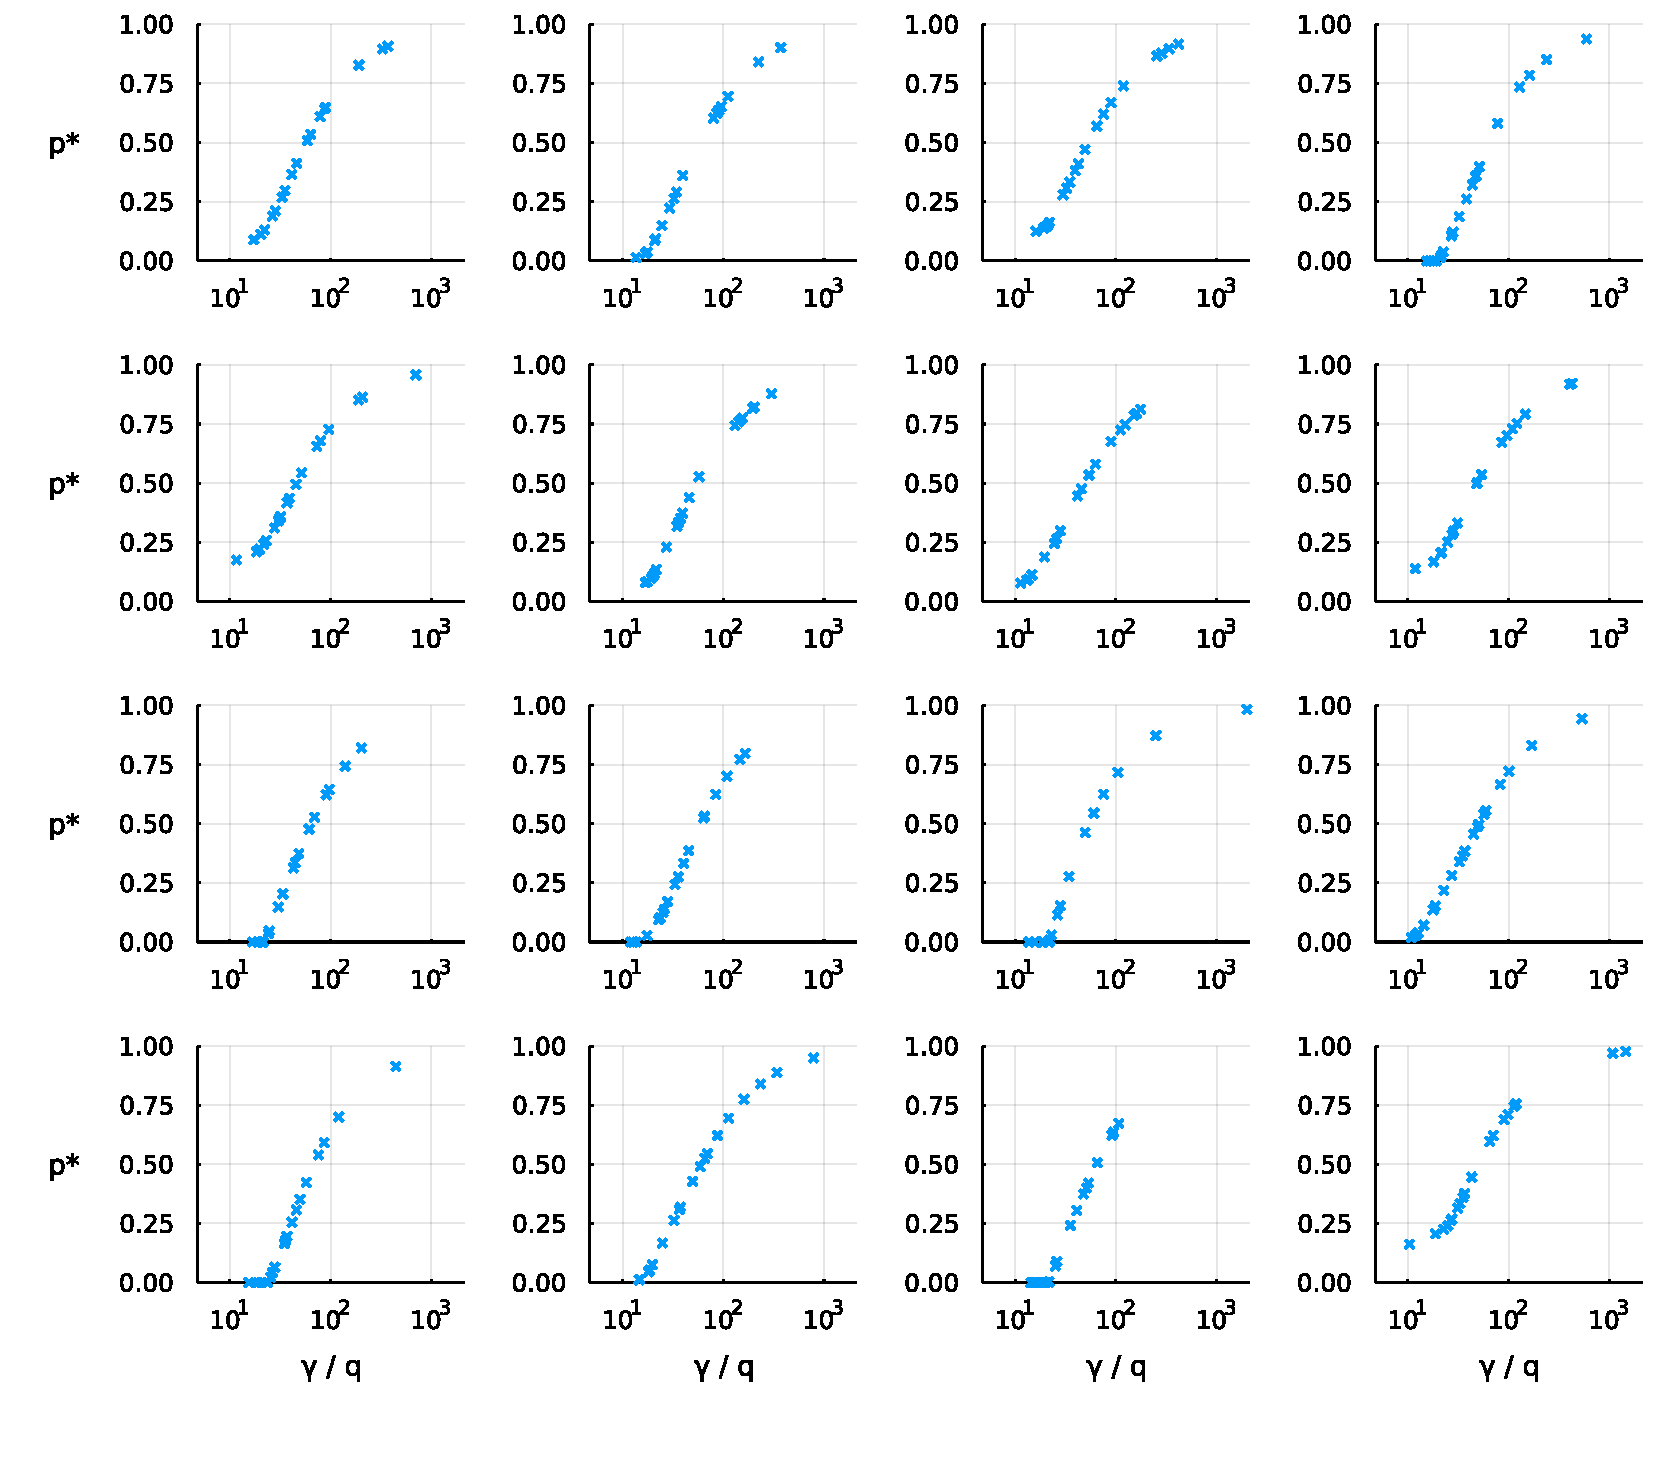
\includegraphics[width=\linewidth, ]{plots/gammaq-pstar.pdf}\end{center}
\captionsetup{singlelinecheck=off}
    \caption[.]{Competitiveness ratios $\gamma_c / q_c$ and equilibrium cutoffs $p_c^*$ in 16 randomly generated admissions markets, each containing 20 schools. The preferability parameters $\delta_c$ are drawn from $\operatorname{Uniform(0, 1)}$, while the capacities are drawn from $\operatorname{Uniform(0, 1/10)}$; hence, the market as a whole has a 50 percent chance of being over- or underdemanded. The figure suggests Theorem \ref{cutoffsortationthm}, which states that the order of the equilibrium cutoffs is determined by the order of competitiveness ratios.}
\label{gammaq-pstar}
\end{figure}

Figures \ref{tat-iter-cutoff} through \ref{score-DA-placement} consider a fictional admissions market called Pallet Town, which has the following parameters. I have sorted the schools by their equilibrium cutoffs.
\begin{gather} \label{pallettowndef}
\begin{aligned}
\gamma &=  \textstyle{\left(\frac{2}{12}, \frac{1}{12}, \frac{3}{12}, \frac{6}{12}\right)}\\
q &= (0.3, 0.1, 0.2, 0.2) \\
p^* &= (0.2, 0.3, 0.4, 0.6)\\
D(p^*, \gamma) &=  (0.3, 0.1, 0.2, 0.2)
\end{aligned}
\end{gather}
As the total capacity is less than one, each school fills its capacity at equilibrium.

Figures \ref{score-cutoff-choice} and \ref{score-DA-placement} consider discrete approximations of the Pallet Town admissions market with samples of 20, 200, and 2000 students. In Figure \ref{score-cutoff-choice}, schools admit students according to their equilibrium cutoffs, students choose their favorite school, and schools observe their demand. When there are many students, the demand at each school approximately equals its capacity. In Figure \ref{score-DA-placement}, a stable matching of the students is computed so that each school fills its capacity exactly. When there are many students, the implied cutoffs approximately equal $p^*$. Compare Figures \ref{score-cutoff-choice} and \ref{score-DA-placement} with figure 4 of Azevedo and Leshno \parencite*{supplydemandfw}, which demonstrates the asymptotic convergence of implicit cutoffs as the number of students increases using a numerical experiment in which scores are partially correlated between schools. 


\begin{figure}
\begin{center}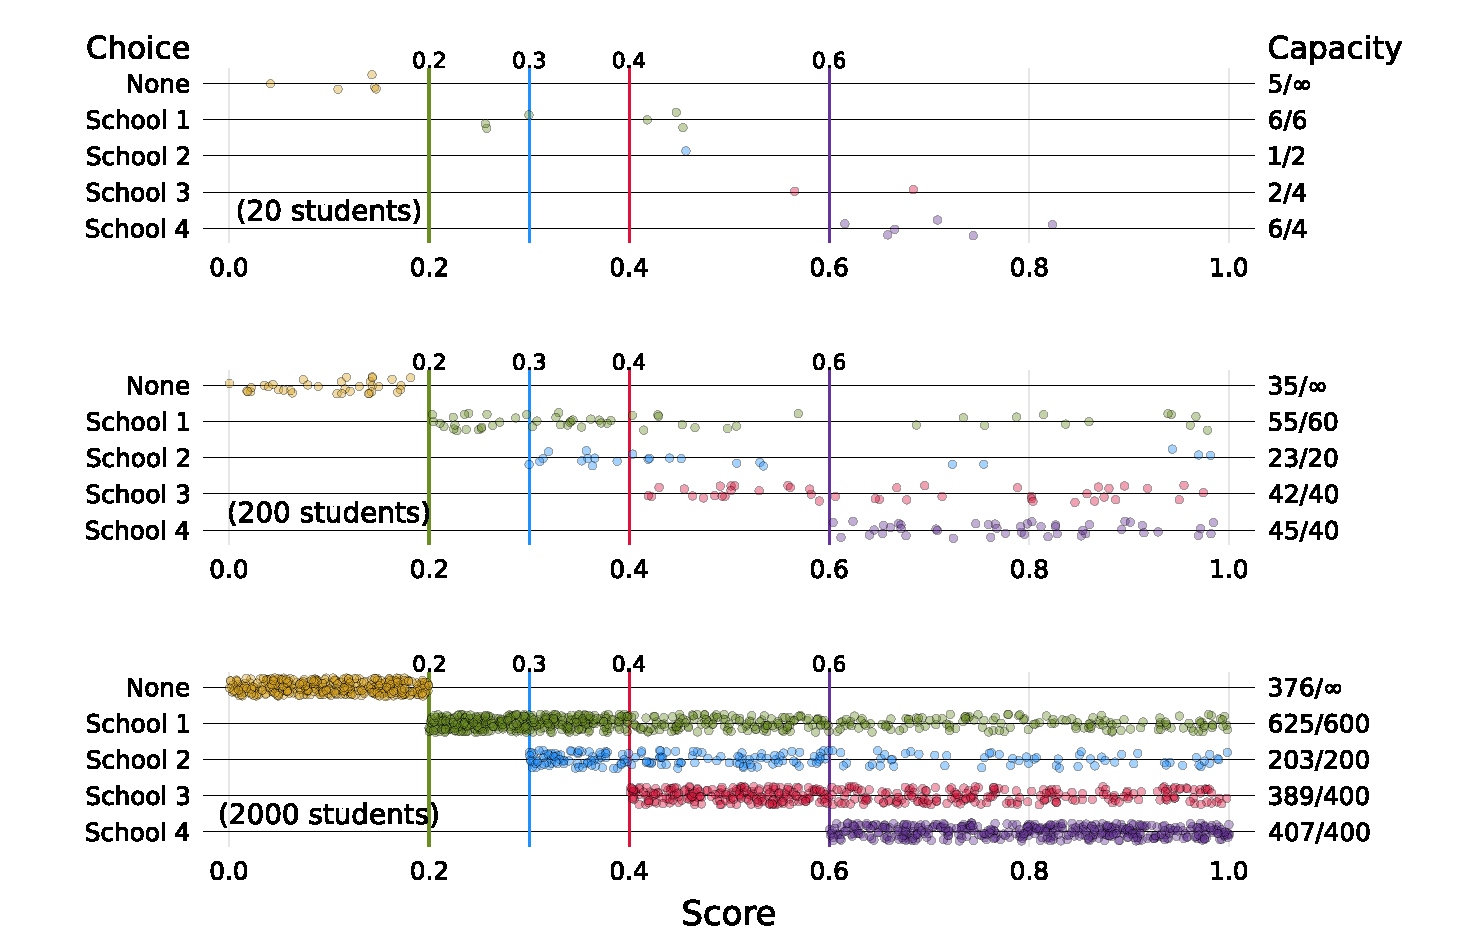
\includegraphics[width=\linewidth, ]{plots/score-cutoff-choice.pdf}\end{center}
\captionsetup{singlelinecheck=off}
    \caption[.]{Simulation of a decentralized school-choice process in Pallet Town. A discrete sample of student preference lists and scores is drawn from $\eta$. Each school admits students whose score exceeds its equilibrium cutoff (shown as vertical lines), then each student chooses her favorite school from her consideration set. As the sample size increases, the demand at each school approximately equals its scaled capacity.}
\label{score-cutoff-choice}
\end{figure}



\begin{figure}
\begin{center}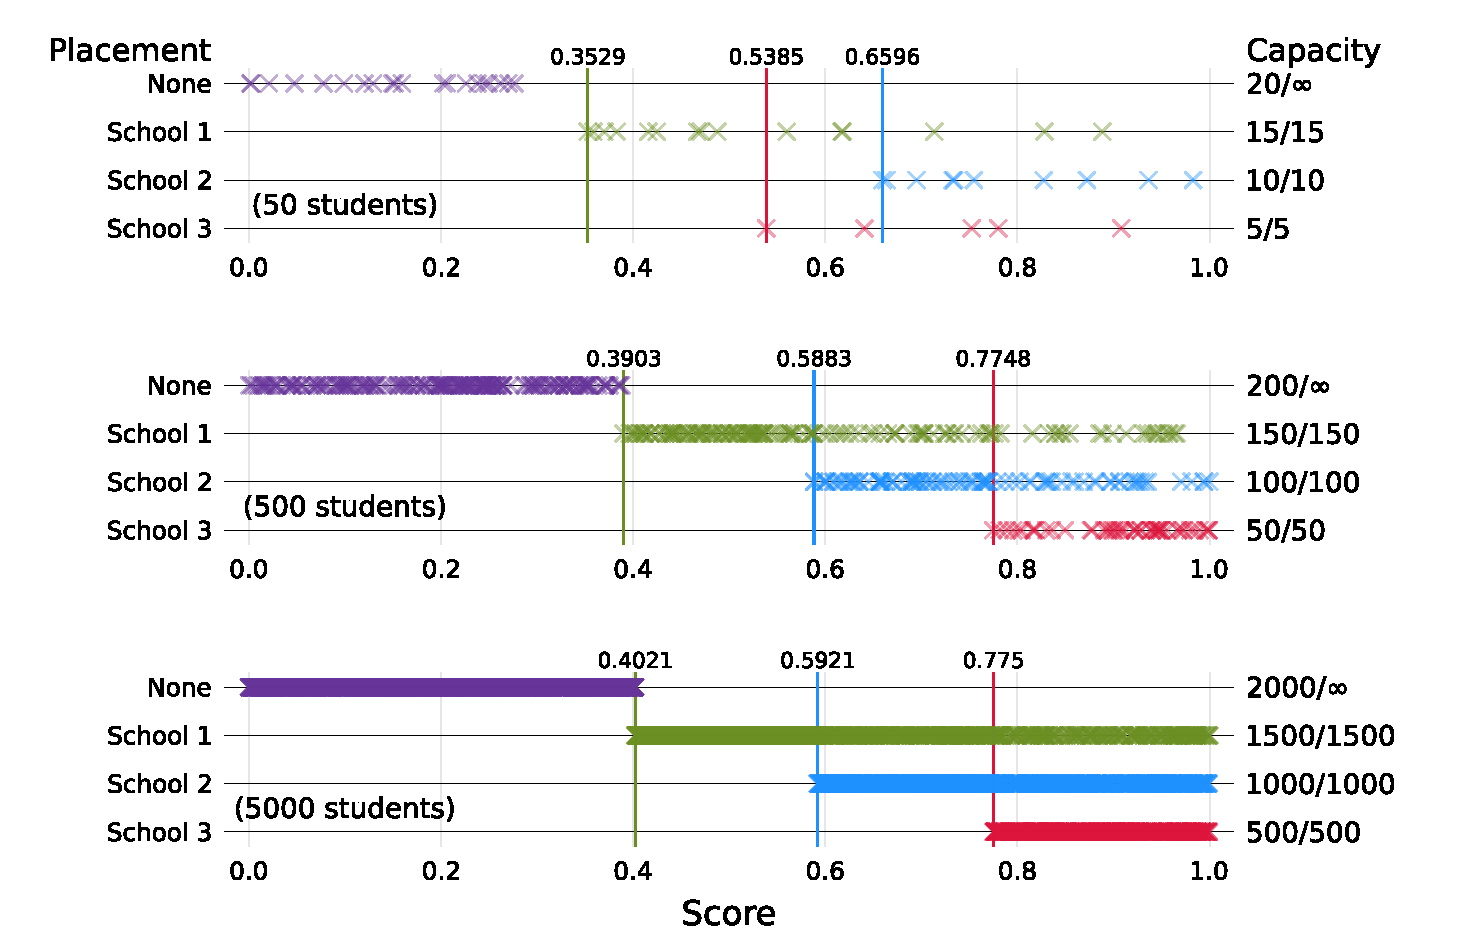
\includegraphics[width=\linewidth, ]{plots/score-DA-placement.pdf}\end{center}
\captionsetup{singlelinecheck=off}
    \caption[.]{Simulation of a deferred acceptance process in Pallet Town. A discrete sample of student preference lists and scores is drawn from $\eta$. The student-proposing deferred acceptance algorithm (Algorithm \ref{studentproposingDA}) is used to compute a stable matching. The score of the least-qualified admit at each school, or the school's implied score cutoff, is computed and represented as a vertical line. Regardless of the sample size, each school fills its scaled capacity, and as the sample size increases, the implied cutoffs approach the market equilibrium. Comparison with Figures \ref{tat-iter-cutoff} and \ref{score-cutoff-choice} suggests the equivalence among stationary points of a t\^{a}tonnement process, market clearing cutoffs, and stable assignments in nonatomic admissions markets.}
\label{score-DA-placement}
\end{figure}


Figures \ref{vary-gamma-demand} and \ref{vary-gamma-cutoff} visualize the incentive analysis under two different assignment paradigms. In Figure \ref{vary-gamma-demand}, the market is decentralized. Suppose that each school would like to achieve higher demand, and that no school is willing to lower cutoff beyond its current value. (For the sake of comparison with the figure that follows, these fixed cutoffs are chosen to equal the equilibrium cutoffs, although the decentralized market allows schools to exceed their capacity.) The four curves in the graph show how each school's demand would respond to a change in each school's $\gamma_c$-value. The slope of each school's quality--demand curve is given by the diagonal of the Jacobian given in equation \eqref{jac-gamma-demand-uncons}. All schools have a positive incentive to improve in quality, and school 2's incentive is the strongest.

Figure \ref{vary-gamma-cutoff} considers a market that is confined to equilibrium, which can be interpreted as a centralized market that uses a DA mechanism or as the equilibrium of a competitive market in which schools' capacities represent target class sizes or hard constraints. In this case, each school is already filled to capacity, so no school has any hope of increasing its demand; instead, suppose that schools hope to increase achieve a higher equilibrium cutoff by increasing their quality. The $y$-axis of the figure shows how each school's equilibrium cutoff responds to an increase in quality; the slope at the current parameters is given by the diagonal of the matrix given in equation \eqref{jac-gamma-p}.

Perhaps the most interesting feature of Figure \ref{vary-gamma-cutoff} is the flat slope at school 1. When the single-score admissions market is confined to equilibrium, the bulk of students who attend school 1 are those who could not obtain admissions anywhere else. A marginal improvement in school 1's quality pulls some students away from more desirable schools, but the \emph{minimum} score of students at school 1 (that is, its cutoff) does not increase until school 1's quality increases to the point that its competitiveness ratio exceeds that of school 2. The plot shows a distinctive set of ``elbows'' where these transitions occur. Visually, these elbows confirm that the market-clearing cutoffs are continuous in the market parameters. 


\begin{figure}
\begin{center}\includegraphics[width=\linewidth, ]{plots/vary-gamma-demand.pdf}\end{center}
\captionsetup{singlelinecheck=off}
    \caption[.]{Quality effects in Pallet Town under a decentralized admissions process like that considered in Figure \ref{score-cutoff-choice}. Each line shows the change in each school’s demand when it changes its quality $\gamma_c$ while holding the cutoff vector and other schools’ quality fixed. To the extent that each school's goal is to increase its demand, the slope of the curve represents the strength the incentive to improve in quality. At the current quality vector, the Jacobian of the demand is
    \begin{equation*}
    \mathbf{J}_\gamma D = A = \frac{1}{360}
    \begin{bmatrix}
22 & -14 & -6&  -2\\
 -7   &29  &-3  &-1\\
 -9   &-9  &15  &-3\\
 -6   &-6&  -6  & 6
    \end{bmatrix}
    \end{equation*} 
    according to the expression provided in \S\ref{unconstrainedqualityeffects}. }
\label{vary-gamma-demand}
\end{figure}






\begin{figure}
\begin{center}\includegraphics[width=\linewidth, ]{plots/vary-gamma-cutoff.pdf}\end{center}
\captionsetup{singlelinecheck=off}
    \caption[.]{Quality effects in Pallet Town under a centralized admissions process such as the deferred acceptance process shown in Figure \ref{score-DA-placement}. Each line shows the change in each school’s equilibrium cutoff when it changes its quality $\gamma_c$ while holding other schools’ quality fixed. To the extent that each school’s objective is increase its cutoff, the slope of the curve represents the strength of the incentive to improve in quality. At the current quality vector, the Jacobian of the equilibrium cutoffs is
    \begin{equation*}
    \mathbf{J}_\gamma \hat p = \frac{1}{30}
    \begin{bmatrix}
      0 & & & \\
      -3 & 6 & & \\
      -2 & -2 & 2 & \\
      -1 & -1 & -1 & 1 
    \end{bmatrix}
    \end{equation*} 
according to the expression derived in \S\ref{qualityeffectsateq}. The elbows in the graph correspond to ties among the competitiveness ratios. 
    }
\label{vary-gamma-cutoff}
\end{figure}








\section{Inverse optimization of single-score admissions markets}
In this section, I consider the inverse optimization task, in which the demand of the market and the cutoff vector is provided and we attempt to compute the quality parameters. I provide an analytic solution, discussion its usefulness to admissions planners, and offer a proof-of-concept demonstration of the inverse optimization task using admissions data from 677 American universities. 

\subsection{The inverse optimization task and an analytic solution}
Given the demand $D$ and cutoff vector $p$, we must solve the following system for $\gamma$.
\begin{equation}
D_c = \sum_{d=c}^{|C|} 
\frac{\gamma_c}{ \sum_{i=1}^d \gamma_i} 
\left(p_{d+1} - p_{d}\right),
\quad \forall c \in C
 \label{solvemeforgamma}
 \end{equation}
Assume the schools are sorted in ascending order of cutoffs, and by homogeneity, let $\sum_{c \in C} \gamma_c \equiv 1$.

Consider the demand for $|C|$, the school with the highest index and therefore highest cutoff. Students who get into this school necessarily get into every school, so the outer sum of the system \eqref{solvemeforgamma} has only one term, and the equation becomes
\begin{align}D_{|C|} =
\frac{\gamma_{|C|}}{ \sum_{i=1}^{|C|} \gamma_i} 
\left(1 - p_{|C|}\right) \\
\implies \gamma_{|C|} = \frac{D_{|C|}}{1 - p_{|C|}}
\end{align}
Now suppose that we know $\gamma_{c+1}, \gamma_{c+2}, \dots, \gamma_{|C|}$. Then $\gamma_c$ can also be calculated from the observation that
\[\sum_{i=1}^d \gamma_i = 1 - \sum_{j=d+1}^{|C|} \gamma_j\]
where I take $\sum_{j=|C|+1}^{|C|} \gamma_j \equiv 0$.

Hence, the following recursive relation allows us to compute all the $\gamma_c$ values in reverse order, starting with $\gamma_{|C|}$ and moving down.\footnote{Because this expression requires repeated division by small numbers, it is numerically unstable when the number of schools is large or there are many schools whose cutoffs are close together or equal. Moreover, the error accumulates with each iteration. Thus, it is sometimes more effective to solve the system \eqref{solvemeforgamma} using a generic root finder; this spreads the numerical error out over all the schools.} 
\begin{align}
\gamma_{|C|} &= \frac{D_{|C|}}{1 - p_{|C|}} \\[1em]
\gamma_c &= \frac{D_c}{~~\mathlarger{\sum_{d=c}^{|C|} \frac{p_{d+1} - p_d}{1 - \sum_{j=d+1}^{|C|} \gamma_j} ~~}}, \quad \forall c \in \bigl\{ |C|-1, |C|-2, \dots, 1\bigr\} \label{gammarecursion}
\end{align}

\subsection{A demonstration using admissions data from American universities}
Here, I demonstrate the inverse optimization process using a public-domain admissions dataset from a large set of American universities \parencite[][]{collegeadmissionskaggle}. The results and discussion below should be taken only as a proof of concept, for four reasons: First, this model makes the unrealistic assumption that all colleges have the same preference order, which is derived from students' standardized test scores. Second, I did not attempt to account for the fact that many students do not bother applying to schools for which they are are overqualified; as a result, the cutoffs are systematic underestimates. Third, the dataset is not adequately sourced, and appears to mix data across years. I used data from the 2017 ACT and 2014 SAT examinations to derive school cutoffs \parencite[][]{ACTprofilerpt, SATpercentileranks}. Finally, I excluded from consideration schools for which test statistics were not listed, reducing the dataset from 1534 schools to 677. Thus, whereas the inverse optimization procedure provided above estimates schools' \emph{preferability} when given perfect knowledge of their \emph{selectivity}, in the present analysis, both quantities had to be estimated.

The dataset contains information regarding four test scores: the critical reading, math, and writing SAT subscores, and ACT composite scores. For each score, the dataset shows the 25th and 75th percentile of scores among students admitted to each school. By comparing these percentiles to percentile tables released by the testing agencies, I derived eight different estimates of each school's cutoff value. For example, at the University of Alabama, the 75th-percentile ACT composite score among admitted students is a 30 (out of 36). Relative to the population of ACT examinees, a student who earns a 30 is at the 90th percentile overall; hence, if the University of Alabama looks only at ACT composite scores, it follows that the minimum score among Alabama's admits is at the 60th percentile among all test-takers. In the occasional case where this calculation yielded a negative value, I cropped it to zero. Explicitly, letting $p_{\text{rel}}$ (here $0.75$) denote the percentile under consideration, and $p_{\text{abs}}$ (here $0.90$) denote the percentile score of a student with that score relative to the whole student population, the implied school cutoff is \[p_{\text{impl}} = \max\left\{0, 1 - \frac{1 - p_{\text{abs}}}{1- p_{\text{rel}}}\right\}\]

To compute a composite estimate of each school's cutoff, I first averaged the cutoffs implied by the ACT and SAT data separately. Then, I took the average of these two weighted by the percentage of applicants who submitted each test score (which is also included in the dataset) and treated this as the school's $p_c$. Schools missing data for any of the eight data points mentioned above were excluded from consideration.

To compute each school's demand, I divided the number of students enrolled at each school by the sum of the same, which is 752,987. Thus, this model assumes that every student in the market can get into at least one college, and that the dataset includes all the college-like options that students in this market would consider. The first assumption is mild, because there are several colleges in the dataset whose estimated cutoff is zero. The second assumption is much more restrictive, as there are many colleges that do not report test scores, not to mention international schools, that are not represented in the data. (In the tabular results and graphs, I report demand as a number of students instead of the proportion $D_c$ for legibility.)

The results are shown in Figure \ref{US-cutoff-gamma} and Table \ref{tab:US-inverse-optimization}. The list of the schools with the highest preferability is a predictable list of prestigious universities. This outcome is remarkable, because the input data contains no explicit indicators of ``prestige'' (such as data on endowment size and employment outcomes), nor any survey data akin to the questionnaires that some newspapers send to college executives to generate their rankings. The model also does not require observations of individual student choices, as used to estimate MNL parameters under traditional statistical paradigms. The preferability parameters simply emerge organically from the selectivity of each school, each school's total demand, and the assumptions about the distribution of student talent. For comparison, Table \ref{tab:US-inverse-optimization} provides other metrics that might be used to assess school preferability such as the demand, cutoff, yield (proportion of admitted students who choose to attend), and \emph{true yield.} The last is a contrived term for the proportion of \emph{qualified} students, regardless of whether they applied, who chose to attend the school; this can be computed from the cutoff and demand. 

Again, due to the low quality of the underlying data, I caution against reading deep meaning into this model's estimates. However, it is worthwhile to take the results at face value for a moment to demonstrate the sort of descriptive analysis enabled by the inverse optimization procedure. 

First, consider the top-ranked schools, whose figures are shown in Table \ref{tab:US-inverse-optimization}. In this market, the top two, Harvard and Yale, appear equally selective (they have almost the same cutoff). However, Harvard achieves a higher preferability parameter because at the same admissions standards, it attracts a larger student body (1659 students, versus Yale's 1356). Conspiciously absent from the list is the school with the highest cutoff, California Institute of Technology ($p_c = 0.9590$, $\gamma_c = 0.0081$, rank 34). While Caltech is a little more selective than Harvard, its entering class size is much smaller, at 249 students. Since, in this model, the set of students admitted to Caltech is only a slight subset of those admitted to Harvard, Harvard must be about $1659 / 249 = 6.7$ times as preferable. Perhaps an admissions director at Caltech would argue that the school's small entering class size is a key element of its appeal, and this is certainly true for many students. However, in this model, Harvard could easily achieve a similar class size to Caltech at a much higher cutoff, eliciting the same conclusion.

 Because this model considers not only selectivity but also entering class size as an indication of market power, compared to conventional college rankings, it grants an elevated position to public flagships like the University of Michigan at Ann Arbor, which draw large entering classes while maintaining fairly high admissions standards. Although tuition price has not figured into any stage of the analysis, this example shows that the computed preferability parameters incorporate a notion of \emph{value,} whereas traditional college rankings arrange schools as if their tuition prices are the same.

It is worth considering schools in other parts of the preferability distribution. While conventional wisdom posits small liberal-arts colleges and large public universities as incommensurable, administrators at both types of school share a common goal of recruiting an entering class that is both ``large'' relative to the physical size of the campus and ``highly qualified'' relative to competitor schools. $\gamma_c$ offers us a way to compare the effectiveness of two schools' marketing efforts even when their recruitment strategies diverge. For example, the University of Vermont and Whitman College (a liberal-arts college in eastern Washington) rank 106th and 107th, with preferability parameters $1.079 \times 10^{-3}$ and $1.044 \times 10^{-3}$, respectively. Vermont has a large class size and a middling cutoff, while Whitman has a small class size and a cutoff close to that of UM Ann Arbor. Looking only at conventional statistics, it is hard to predict the decision of a student choosing between the two schools, but comparing $\gamma$-values (which are, by definition, choice probability weights) reveals that in this case it is a nearly even coin flip. Indeed, the two school's demand curves (shown in Figure \ref{three-demand-curves}) are all but identical. 

The inverse optimization task makes no equilibrium assumption, and indeed invokes no notion of capacity or target class size. It simply reports the status of the market with respect to the current allocation of students. Thus, a possible application of this model is for an admissions director to use in modeling her school's demand curve. Figure \ref{three-demand-curves} shows the predicted demand curves for Vermont, Whitman, and Caltech. In the future, suppose that Caltech decides that a larger cohort of 350 students better suits its goals. By how much should it relax its admissions standards in order to achieve this class size? One way to answer this question is to assume that Caltech’s true yield remains approximately fixed. Then, Caltech should try to become $\frac{350}{249}$ as selective, by updating its cutoff to $1 - \frac{350}{249}(1 - 0.9590) = 0.9424$. A simple calculation shows that this way of estimating the demand curve is equivalent to fitting a linear model to the observed demand $(p_c, D_c) = (.9590, 249)$ and the implicit $x$-intercept $(1, 0)$. 

However, when using a linear model, the recommended cutoff associated with the higher target demand will be a slight underestimate, because Caltech’s true yield also varies as a function of $p$. Under the recommended cutoff, students admitted with scores of (say) $0.95$ do \emph{not} qualify for Harvard and Yale, so Caltech will not have to compete as fiercely to recruit them as it does to recruit its current enrollees. The model presented here accounts for this change in the consideration set of marginal students, and thus calls for a more modest reduction in Caltech’s cutoff, to the value of $0.9437$.

Figure \ref{caltech-demand-curve} presents a detailed view of Caltech’s demand curve as predicted by this model alongside the linear model. The curve has a slightly bowed shape, which confirms the intuitive argument for a gentler relaxation of admissions standards in order to achieve lower target enrollment. In fact, every school’s demand curve in this model is piecewise linear convex, meaning that linear regression will always underestimate the demand at cutoffs far from those used to fit the line.\footnote{If the linear model is constrained to contain the point $(1, 0)$, then it forms a chord of the convex curve, and it will \emph{overestimate} the demand at $p_c$-values \emph{higher} than those used to fit the model. On the other hand, if this constraint is dropped and the model is fitted to two or more local observations, then it will \emph{underestimate} the demand at both higher and lower cutoffs.} Of course, a more accurate regression could be constructed by using demand observations from multiple years and including a quadratic term. But even then, if the observations used to fit the curve remain in the same ``piece'' of the piecewise linear demand function, then the expected regression curve will be a straight line.

This analysis has not accounted for the hypothesis that Caltech's appeal depends on a small class size, in which case looser admissions standards also reduce the school's preferability, necessitating a lower cutoff after all. Thus, in practical decisionmaking a model like that presented here is unlikely to be competitive with colleges' in-house models, which incorporate specific observations of students who applied to the school and chose to attend another. However, an advantage of the current model is that it produces an informative approximation of the demand curve without using students' personal data. Thus, a school like Caltech can use it to model the demand curves of its \emph{competitors} schools, enabling a more sophisticated recruitment strategy. 

\begin{figure}
\begin{center}\includegraphics[width=\linewidth, ]{plots/US-cutoff-gamma.pdf}\end{center}
\captionsetup{singlelinecheck=off}
    \caption[.]{Inverse optimization procedure applied to a dataset of 677 American universities. School cutoffs were determined using a weighted average of cutoffs inferred from admitted students' SAT and ACT scores at the 25th and 75th percentiles. The marker size indicates the true yield, or percentage of qualified students who choose to attend each school. Details for the top twenty schools, as ranked by $\gamma_c$, appear in Table \ref{tab:US-inverse-optimization}.}
\label{US-cutoff-gamma}
\end{figure}




\begin{table}[]
\begin{tabular}{r|l|r|l|l|l|l}
\multicolumn{1}{l|}{\textbf{Rank}} & \textbf{University}                   & \multicolumn{1}{l|}{\textbf{Demand}} & \textbf{\begin{tabular}[c]{@{}l@{}}Cutoff\\ ($p_c$)\end{tabular}} & \textbf{Yield} & \textbf{True yield} & \textbf{\begin{tabular}[c]{@{}l@{}}Preferability\\ ($\gamma_c$)\end{tabular}} \\ \hline
1                                  & Harvard U                             & 1659                                 & 0.9526                  & 0.81           & 0.0465              & 0.0465                              \\
2                                  & Yale U                                & 1356                                 & 0.9527                  & 0.66           & 0.0381              & 0.0381                              \\
3                                  & U of Chicago                          & 1426                                 & 0.949                   & 0.53           & 0.0371              & 0.0367                              \\
4                                  & U of Pennsylvania                     & 2421                                 & 0.9207                  & 0.63           & 0.0405              & 0.0358                              \\
5                                  & Northwestern U                        & 2037                                 & 0.9268                  & 0.41           & 0.0369              & 0.0337                              \\
6                                  & Cornell U                             & 3223                                 & 0.8984                  & 0.52           & 0.0421              & 0.0326                              \\
7                                  & Washington U in St. Louis              & 1610                                 & 0.9364                  & 0.34           & 0.0336              & 0.032                               \\
8                                  & Mass. Institute of Technology & 1115                                 & 0.9515                  & 0.72           & 0.0305              & 0.0304                              \\
9                                  & Princeton U                           & 1285                                 & 0.9445                  & 0.65           & 0.0308              & 0.03                                \\
10                                 & Stanford U                            & 1677                                 & 0.9307                  & 0.76           & 0.0321              & 0.0299                              \\
11                                 & Vanderbilt U                          & 1613                                 & 0.932                   & 0.41           & 0.0315              & 0.0295                              \\
12                                 & Columbia U    & 1415                                 & 0.9338                  & 0.6            & 0.0284              & 0.0268                              \\
13                                 & Duke U                                & 1714                                 & 0.918                   & 0.42           & 0.0278              & 0.0242                              \\
14                                 & U of Michigan--Ann Arbor               & 6200                                 & 0.813                   & 0.4            & 0.044               & 0.0228                              \\
15                                 & New York U                            & 5207                                 & 0.8256                  & 0.35           & 0.0397              & 0.0218                              \\
16                                 & Northeastern U                        & 2891                                 & 0.864                   & 0.19           & 0.0282              & 0.0182                              \\
17                                 & Brown U                               & 1543                                 & 0.9065                  & 0.58           & 0.0219              & 0.0178                              \\
18                                 & U of California--Berkeley              & 4162                                 & 0.8214                  & 0.37           & 0.0309              & 0.0167                              \\
19                                 & U of Southern California              & 2922                                 & 0.8509                  & 0.31           & 0.026               & 0.0159                              \\
20                                 & Carnegie Mellon U                     & 1442                                 & 0.9035                  & 0.3            & 0.0198              & 0.0158                             
\end{tabular}
\caption{\label{tab:US-inverse-optimization}
The top twenty schools by preferability $\gamma_c$, as determined by applying the inverse optimization process to a dataset of 677 American universities. Each school's demand is given as the number of students in the entering class; to compute $D_c$, divide by the total number of students, 752,987. The school's yield is as reported by the admissions office, while the true yield, which represents the proportion of qualified students who chose to attend the school, was computed by comparing the size of the entering class to the estimated cutoff $p_c$.}
\end{table}





\begin{figure}
\begin{center}\includegraphics[width=\linewidth, ]{plots/three-demand-curves.pdf}\end{center}
\captionsetup{singlelinecheck=off}
    \caption[.]{Three demand curves derived via the inverse optimization process. The University of Vermont and Whitman College have similar preferability parameters, and thus similar demand curves. However, each school has chosen a different selectivity threshold, reflecting its distinct admissions priorities. A detailed view of Caltech's demand curve appears in Figure \ref{caltech-demand-curve}.}
\label{three-demand-curves}
\end{figure}





\begin{figure}
\begin{center}\includegraphics[width=\linewidth, ]{plots/caltech-demand-curve.pdf}\end{center}
\captionsetup{singlelinecheck=off}
    \caption[.]{Detailed view of Caltech's demand curve near its current cutoff. Assuming preferability and other schools' cutoffs remain fixed, if Caltech wishes to increase its class size to 350, it should update its cutoff to the value indicated by the intersection of the demand curve and the horizontal coral line. A linear model prescribes decreasing the cutoff to $p_c = 0.9424$, whereas the model provided here accounts for the fact that there is less competition for marginal students at the lower cutoff and prescribes a more conservative decrease to $0.9437$. }
\label{caltech-demand-curve}
\end{figure}








The code used to produce these results, as well as more details regarding how the cutoffs were estimated from available SAT and ACT data, is available on GitHub \parencite[][]{studentprefsrevopt}.



\subsection{The informational quality of $\gamma$, and the bias in (true) yield}
The question of how to measure aggregate college preferability is not a simple one, and newspaper university rankings attract regular controversy for their imprecise methodology \parencite[][]{intlrankingsandconflicts}. Typical ranking metrics draw from a combination of survey data and performance measures of a university's quality such as its research output or data on alumni salaries. However, conducting accurate surveys is costly and difficult, and while performance measures may correlate with college preferability, they offer a normative indication of which colleges ``should'' be popular without accounting for the decisions students actually make---decisions that may depend less on hard facts than on intangible notions of fitness.

The traditional measure college administrators have used to quantify how preferable their school is relative to others in the market has been the yield. As discussed above, colleges' \emph{true} yield (or another yield metric that corrects for applicant behavior) can be a useful tool in modeling the demand curve. However, as a measure of comparing the preferability of two different colleges, true yield systematically overrates lenient schools, which face less competition for students. For example, consider a market with only two schools, Lunar College ($p_1 = 0, D_1 =  \frac{100}{101}$) and Antarctic University ($p_2 = \frac{99}{100}, D_2 = \frac{1}{101}$). At both schools, the true yield is $D_c / (1 - p_c) = \frac{100}{101}$, a value which exaggerates the preferability of Lunar College by failing to account for the fact that the majority of its admits, and the vast majority of its enrollees, had no other option. The proportion of students who chose Lunar College \emph{over} Antarctic University is given by the former's preferability, $\gamma_1 = \frac{100/101 - 99/100}{1/100} = \frac{1}{101}$, while the preferability of Antartic University is $\gamma_2 = \frac{100}{101}$. This example, along with the demonstration above, suggests that insofar as $\gamma$ can be estimated accurately, it provides unbiased information about school preferability in a well-differentiated admissions market.

\section{Discussion}
This article has considered the characterization of nonatomic admissions markets, and attempted to incorporate the best elements of the mechanism-design paradigm that treats stable assignment as a normative goal alongside those of regression models that parameterize colleges' demand in a decentralized context. Under the assumption that each school's capacity in the school-choice problem can be interpreted as its target demand, stable matchings produced by DA mechanisms coincide with competitive equilbria of decentralized admissions markets. While this interpretation readily follows from prior results, I have also argued that each iteration of DA mechanisms can be characterized by the price vector, and thus that DA is a special form of t\^{a}tonnement. Thus, given access to an oracle that computes the demand for each school at a given cutoff vector, equilibrium cutoffs can be efficiently computed using a generic t\^{a}tonnement algorithm.

One interpretation of the relationship between discrete admissions markets (with a finite collection of students and integral school capacities) and nonatomic admissions markets (with a distribution over the set of student types and fractional school capacities) regards instances of the former as samples from the latter. Hence, if the parameters of a given economy are known, then computing equilibria and comparative statics with respect to the nonatomic formulation offers a picture of the expected behavior of the market that is insensitive to discretization error. Unfortunately, as shown in this paper's first section, the endogenous complexity of the space of student types makes nonatomic markets difficult to work with directly. Thus, constructing the oracle mentioned in the previous paragraph is usually difficult, and there remains no general solution to the problem of finding equilibrium cutoffs in an arbitrary nonatomic market.

Nonetheless, by making simplifying assumptions on schools' scoring practices and choosing a suitable parametric choice model, we can sometimes compute the demand efficiently. In the example considered here, students choose schools according to a multinomial logit function and schools share a common scoring procedure. Then an invertible, piecewise linear expression relates the market parameters $\gamma$, $D$, and $p$. Though this model is rather simplistic, solving for the preference parameters $\gamma$ using real data from a set of American colleges produced an intuitive ordering of top universities. The model also allows the analyst to chart each school's demand curve without consulting granular data on individual students' enrollment decisions or assumptions about either set of players' utility functions. 

\subsection{Future directions}
Natural extensions of the computational model considered here include the mixed MNL model and mixed scoring vectors. Both of these modifications would allow for differentiation based on students' academic interests; for example, students interested in the performing arts systematically promote conservatories in their preference orders, and these schools in turn will score applicants according to different criteria. However, any departure from the single scoring model invites rapid multiplication in the number of possible consideration sets, in principle because it becomes impossible to construct a total ordering of the space of students. Further upstream sits the question of how to evaluate student ability in the first place. Modern standardized examinations used to assess school performance are weighted by individual and school characteristics, and the scoring formula treats the high-dimensional concatenation of student responses, rather than simply the number of correct answers, as the explanatory variable of ability \parencite[][]{measurementofstudentability}. These devices complicate the analyst's task.

A more robust account of the notion of equilibrium in decentralized admissions markets is also needed. This paper's definition of equilibrium was chosen because it coincides with stable assignments, but in principle, schools can have arbitrary utility functions, and the equilibrium in general nonatomic admissions markets will seldom agree with the stable assignment produced by a centralized mechanism. Furthermore, real schools' preferences may be cardinal rather than ordinal, and are sensitive to the composition of the entering class along with its summary statistics, as pointed out by Roth \parencite*{collegeadmissionsisnotmarriage}. Thus, the results given in this paper cannot fully predict the relative efficiency and fairness of decentralized admissions procedures. 

However, in the real world, putatively decentralized admissions procedures often incorporate regulatory elements that push the market toward stable assignment. For example, the college admissions procedure in South Korea can be viewed as a distributed approximation of school-proposing DA. In this model, the government places a firm limit, called an admissions quota, $q_c$ on the number of students who can attend each university. At the beginning of the admissions cycle, colleges are given the profiles of all the students interested in attending. Each college makes admissions offers over the course of several rounds, beginning with the highest-qualified students, and at each round a subset of the admitted students tentatively commits to attending one of the colleges that admitted them. This process continuous for three rounds, at which point most colleges have either filled their capacity, or bottomed out their pool of applicants. If students were allowed to apply to every college and there were infinite rounds, this would be equivalent to school-proposing DA. However, students are in fact allowed to apply to only six colleges, and colleges instate different evaluation criteria for students who rank the school with high priority. It would be interesting to quantify the welfare cost of these regulations relative to a true stable assignment procedure. The MNL model with single scoring could be a useful analytic tool, because admissions decisions in Korea are based heavily on standardized test scores, and the market is well differentiated vertically.

This article has taken a microeconomic view of admissions markets that views the market as a closed system in which the set of schools and the distribution of student preferences are frozen. Thus, the results offered here are incommensurate with macroeconomic studies in the so-called Tiebout framework that model the sorting behavior of families who move in and out of admissions markets according to how much they value public education overall \parencite[][]{apuretheoryoflocalexpenditures, equilibriumandlocalredistribution}. Because this area of the literature includes comparisons across districts that use different assignment mechanisms, it would be worthwhile to examine the relationship between sorting behavior and choice mechanisms, whereas previous regression studies have treated sorting behavior as a dependent variable that must be controlled for \parencite[][]{doescompetitionamongpublicschools}.

\pagebreak
\section{References}
\printbibliography[heading=none]

\end{document}

